\documentclass[journal]{IEEEtran}

% For revision control
\usepackage{rcs-multi}
\rcsid{$Id$}
\rcsid{$Header$}
\rcskwsave{$Author$}
\rcskwsave{$Date$} 
\rcskwsave{$Revision$}
%%\rcsRegisterAuthor{devangel}{Dennis Jos{\'e} Evangelista}
\rcsRegisterAuthor{devangel}{Dennis J. Evangelista}



\usepackage{cite}
\usepackage{graphicx}
\usepackage[usenames,dvipsnames]{color}
\usepackage{makeidx}

% PDF metadata
\usepackage{hyperref}
\hypersetup{pdftitle={}}
\hypersetup{pdfauthor={Kevin Peterson, some guys, Dennis Evangelista}}
\hypersetup{pdfsubject={biology}}
\hypersetup{pdfkeywords={biomechanics}}
\hypersetup{colorlinks=true,citecolor=Violet,linkcolor=Blue,urlcolor=Red}


\usepackage[cmex10]{amsmath}
% Also, note that the amsmath package sets \interdisplaylinepenalty to 10000
% thus preventing page breaks from occurring within multiline equations. Use:
\interdisplaylinepenalty=2500
% after loading amsmath to restore such page breaks as IEEEtran.cls normally
% does.

%\usepackage{array} % ONE OF THESE CONFLICTS WITH SIUNITX
%\usepackage{mdwmath}
%\usepackage{mdwtab}
% IEEEtran contains the IEEEeqnarray family of commands that can be used to
% generate multiline equations as well as matrices, tables, etc., of high
% quality.

% correct bad hyphenation here
\hyphenation{op-tical net-works semi-conduc-tor}

% use default cite for IEEE styles
\bibliographystyle{IEEEtran}
%\usepackage[round]{natbib}
%\setcitestyle{authoryear, round, comma, aysep={;}, yysep={,}, notesep={, }}
%\bibliographystyle{apalike}

% Genus and species names
\newcommand{\PHAT}{PHAT}
\newcommand{\Calypteanna}{\emph{Calypte anna}}

\usepackage{siunitx}

\begin{document}
\title{Flapping tails}

\author{Kevin Peterson,
		Some Guys,
	    Dennis~Evangelista,~\IEEEmembership{Member,~IEEE,}
\thanks{Dennis Evangelista is with the Department
of Integrative Biology, University of California, Berkeley, CA, 94720-3140 USA e-mail: devangel@berkeley.edu}% <-this % stops a space
\thanks{Kevin Peterson is with the Department of Electrical Engineering and Computer Science, University of California, Berkeley, CA, 94720-3140.}% <-this % stops a space
\thanks{Manuscript received \today; revised some day later.}}

% The paper headers
\markboth{Journal of \LaTeX\ Class Files,~Vol.~6, No.~1, January~2007}%
{Evangelista \MakeLowercase{\textit{et al.}}: iFAPALOT}

%\IEEEpubid{0000--0000/00\$00.00~\copyright~2007 IEEE}
% Remember, if you use this you must call \IEEEpubidadjcol in the second
% column for its text to clear the IEEEpubid mark.
% use for special paper notices
%\IEEEspecialpapernotice{(Invited Paper)}




% make the title area
\maketitle

\begin{abstract}
Abstract here copy from learning contracts
\end{abstract}

% Note that keywords are not normally used for peerreview papers.
\begin{IEEEkeywords}
flight, tails
\end{IEEEkeywords}

\IEEEpeerreviewmaketitle



\section{Introduction}
% The very first letter is a 2 line initial drop letter followed
% by the rest of the first word in caps.
% 
% form to use if the first word consists of a single letter:
% \IEEEPARstart{A}{demo} file is ....
% 
% form to use if you need the single drop letter followed by
% normal text (unknown if ever used by IEEE):
% \IEEEPARstart{A}{}demo file is ....
% 
% Some journals put the first two words in caps:
% \IEEEPARstart{T}{his demo} file is ....
% 
% Here we have the typical use of a "T" for an initial drop letter
% and "HIS" in caps to complete the first word.
\IEEEPARstart{T}{his} demo file is intended to serve as a ``starter file''
for IEEE journal papers produced under \LaTeX\ using
IEEEtran.cls version 1.7 and later.
% You must have at least 2 lines in the paragraph with the drop letter
% (should never be an issue)
I wish you the best of success.

% needed in second column of first page if using \IEEEpubid
%\IEEEpubidadjcol
\subsection{Biological inspiration for tail designs}
\subsection{Base robot}
\subsection{Study goals: biology and robot design}

\section{Tail design and construction}
You probably need to explain how you designed and built the tails.
\begin{figure}
\caption{Hello array.}
\label{fig:intro}
\end{figure}
 
\section{Flight test methodology}
Then you need to explain how they were tested.

\section{Flight test results}
The test results go here. 

\section{Conclusion}
Everything works beautifully all the time. Explain the next steps about how this would be used in a real application. Also explain what this tells the biologists about how flight might have evolved. 




% use section* for acknowledgement
\section*{Acknowledgment}

For their support and valuable discussions, we thank people... We also thank Tom Libby, Evan Chang-Siu, and the Berkeley Center for Integrative Biomechanics Education and Research (CIBER) for use of tools and equipment.  


% Can use something like this to put references on a page
% by themselves when using endfloat and the captionsoff option.
\ifCLASSOPTIONcaptionsoff
  \newpage
\fi



% trigger a \newpage just before the given reference
% number - used to balance the columns on the last page
% adjust value as needed - may need to be readjusted if
% the document is modified later
%\IEEEtriggeratref{8}
% The "triggered" command can be changed if desired:
%\IEEEtriggercmd{\enlargethispage{-5in}}

% references section
\nocite{Mueller:2002}
\bibliography{references/flapping-tails}












% biography section
% 
% If you have an EPS/PDF photo (graphicx package needed) extra braces are
% needed around the contents of the optional argument to biography to prevent
% the LaTeX parser from getting confused when it sees the complicated
% \includegraphics command within an optional argument. (You could create
% your own custom macro containing the \includegraphics command to make things
% simpler here.)
%\begin{biography}[{\includegraphics[width=1in,height=1.25in,clip,keepaspectratio]{mshell}}]{Michael Shell}
% or if you just want to reserve a space for a photo:


%\begin{IEEEbiography}{Dennis Evangelista}
\begin{IEEEbiography}[{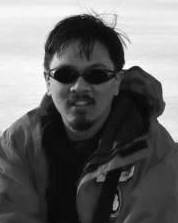
\includegraphics[width=1in,height=1.25in]{figures/blurb-photos/evangelista.jpg}}]{Dennis Evangelista}
Dennis Evangelista is currently a Ph.D.\ candidate in the Department of Integrative Biology at UC Berkeley.  Dennis earned the BSME, BSEE, and MEng EECS degrees from MIT in 1999; and the MSES ME degree from Naval Postgraduate School in 2001.  Dennis previously served as a lieutenant in the United States Navy, where he was assigned as a nuclear engineer at Naval Sea Systems Command / Naval Reactors. He is a licensed professional engineer. His current biological research interests include flight biomechanics, locomotion and control of locomotion in variable environments, fast movements in plants, ecomechanics, biomechanics in evolution, and the design of instrumentation for organismal studies.  
\end{IEEEbiography}

% if you will not have a photo at all:
\begin{IEEEbiography}{Kevin Peterson}
Virgina Tech is cool. 
\end{IEEEbiography}

% insert where needed to balance the two columns on the last page with
% biographies
%\newpage

% You can push biographies down or up by placing
% a \vfill before or after them. The appropriate
% use of \vfill depends on what kind of text is
% on the last page and whether or not the columns
% are being equalized.

\vfill

% Can be used to pull up biographies so that the bottom of the last one
% is flush with the other column.
%\enlargethispage{-5in}

% that's all folks
\end{document}






% An example of a floating figure using the graphicx package.
% Note that \label must occur AFTER (or within) \caption.
% For figures, \caption should occur after the \includegraphics.
% Note that IEEEtran v1.7 and later has special internal code that
% is designed to preserve the operation of \label within \caption
% even when the captionsoff option is in effect. However, because
% of issues like this, it may be the safest practice to put all your
% \label just after \caption rather than within \caption{}.
%
% Reminder: the "draftcls" or "draftclsnofoot", not "draft", class
% option should be used if it is desired that the figures are to be
% displayed while in draft mode.
%
%\begin{figure}[!t]
%\centering
%\includegraphics[width=2.5in]{myfigure}
% where an .eps filename suffix will be assumed under latex, 
% and a .pdf suffix will be assumed for pdflatex; or what has been declared
% via \DeclareGraphicsExtensions.
%\caption{Simulation Results}
%\label{fig_sim}
%\end{figure}

% Note that IEEE typically puts floats only at the top, even when this
% results in a large percentage of a column being occupied by floats.


% An example of a double column floating figure using two subfigures.
% (The subfig.sty package must be loaded for this to work.)
% The subfigure \label commands are set within each subfloat command, the
% \label for the overall figure must come after \caption.
% \hfil must be used as a separator to get equal spacing.
% The subfigure.sty package works much the same way, except \subfigure is
% used instead of \subfloat.
%
%\begin{figure*}[!t]
%\centerline{\subfloat[Case I]\includegraphics[width=2.5in]{subfigcase1}%
%\label{fig_first_case}}
%\hfil
%\subfloat[Case II]{\includegraphics[width=2.5in]{subfigcase2}%
%\label{fig_second_case}}}
%\caption{Simulation results}
%\label{fig_sim}
%\end{figure*}
%
% Note that often IEEE papers with subfigures do not employ subfigure
% captions (using the optional argument to \subfloat), but instead will
% reference/describe all of them (a), (b), etc., within the main caption.


% An example of a floating table. Note that, for IEEE style tables, the 
% \caption command should come BEFORE the table. Table text will default to
% \footnotesize as IEEE normally uses this smaller font for tables.
% The \label must come after \caption as always.
%
%\begin{table}[!t]
%% increase table row spacing, adjust to taste
%\renewcommand{\arraystretch}{1.3}
% if using array.sty, it might be a good idea to tweak the value of
% \extrarowheight as needed to properly center the text within the cells
%\caption{An Example of a Table}
%\label{table_example}
%\centering
%% Some packages, such as MDW tools, offer better commands for making tables
%% than the plain LaTeX2e tabular which is used here.
%\begin{tabular}{|c||c|}
%\hline
%One & Two\\
%\hline
%Three & Four\\
%\hline
%\end{tabular}
%\end{table}


% Note that IEEE does not put floats in the very first column - or typically
% anywhere on the first page for that matter. Also, in-text middle ("here")
% positioning is not used. Most IEEE journals use top floats exclusively.
% Note that, LaTeX2e, unlike IEEE journals, places footnotes above bottom
% floats. This can be corrected via the \fnbelowfloat command of the
% stfloats package.






% if have a single appendix:
%\appendix[Proof of the Zonklar Equations]
% or
%\appendix  % for no appendix heading
% do not use \section anymore after \appendix, only \section*
% is possibly needed

% use appendices with more than one appendix
% then use \section to start each appendix
% you must declare a \section before using any
% \subsection or using \label (\appendices by itself
% starts a section numbered zero.)
%
%
%\appendices
%\section{Proof of the First Zonklar Equation}
%Appendix one text goes here.
%
%% you can choose not to have a title for an appendix
%% if you want by leaving the argument blank
%\section{}
%Appendix two text goes here.
%